\documentclass[10pt]{article}
\usepackage{ctex} % 中文支持
\usepackage{titling} % 标题格式定制
\usepackage{lipsum} % 示例文本
\usepackage{titlesec} % 标题格式定制
\usepackage{graphicx}
\usepackage{amssymb}
\usepackage{float}
\usepackage{array}
\usepackage{color}
\usepackage{geometry}
\usepackage{amsmath}
\usepackage{textcomp}
\geometry{left=2.5cm,right=2.5cm,top=2.0cm,bottom=2.0cm}

% 设置标题格式
\titleformat{\section}{\centering\Large\bfseries}{\thesection}{1em}{}
\titleformat{\subsection}{\centering\large\bfseries}{\thesubsection}{1em}{}
\titleformat{\subsubsection}{\centering\normalsize\bfseries}{\thesubsubsection}{1em}{}

% 调整标题位置
\setlength{\droptitle}{-2cm}

\begin{document}

\title{\huge{\textbf{2024秋数值代数-实验报告\#5}}}
\author{姓名:\underline{李奕萱} \hspace{1cm}学号:\underline{PB22000161} }
\date{\today}

\maketitle

运行环境:\underline{win11,vscode,py3}

\section{实验内容与要求}

\textcolor{blue}{\textbf{利用最小二乘法预测未来人口}}

$ $

下表为最近若干年的人口数据

\begin{table}[H]
\centering
\small
\begin{tabular}{
  |>{\centering\arraybackslash}p{0.65cm}
  |>{\centering\arraybackslash}p{1cm}
  |>{\centering\arraybackslash}p{1.3cm}
  |>{\centering\arraybackslash}p{1.3cm}
  |>{\centering\arraybackslash}p{1cm}
  |>{\centering\arraybackslash}p{1cm}
  |>{\centering\arraybackslash}p{1.3cm}
  |>{\centering\arraybackslash}p{1.3cm}
  |>{\centering\arraybackslash}p{1.3cm}
  |}
\hline
\textbf{年份} & \textbf{总人口(亿人)} & \textbf{出生人口(万人)} & \textbf{死亡人口(万人)} & \textbf{出生率(\textperthousand)} & \textbf{死亡率(\textperthousand)} & \textbf{城镇人口(亿人)} & \textbf{乡村人口(亿人)} & \textbf{城镇化率(\textperthousand)} \\
\hline
2010 & 13.4091 & 1588 & 948 & 11.84 & 7.07 & 6.6978 & 6.7113 & 49.9 \\ \hline
2011 & 13.4916 & 1599 & 957 & 11.85 & 7.09 & 6.9927 & 6.4989 & 51.8 \\ \hline
2012 & 13.5922 & 1630 & 966 & 11.99 & 7.11 & 7.2175 & 6.3747 & 53.1 \\ \hline
2013 & 13.6726 & 1635 & 969 & 11.96 & 7.09 & 7.4502 & 6.2224 & 54.5 \\ \hline
2014 & 13.7646 & 1683 & 974 & 12.23 & 7.08 & 7.6738 & 6.0908 & 55.8 \\ \hline
2015 & 13.8326 & 1655 & 975 & 11.96 & 7.05 & 7.9302 & 5.9024 & 57.3 \\ \hline
2016 & 13.9232 & 1786 & 977 & 12.83 & 7.02 & 8.1924 & 5.7308 & 58.8 \\ \hline
2017 & 14.0011 & 1723 & 986 & 12.31 & 7.04 & 8.4343 & 5.5688 & 60.2 \\ \hline
2018 & 14.0541 & 1523 & 993 & 10.84 & 7.07 & 8.6433 & 5.4108 & 61.5 \\ \hline
2019 & 14.1008 & 1465 & 998 & 10.39 & 7.05 & 8.8426 & 5.2582 & 62.7 \\ \hline
2020 & 14.1212 & 1202 & 997.6 & 8.51 & 7.06 & 9.022 & 5.0992 & 63.9 \\ \hline
2021 & 14.1260 & 1062 & 1014 & 7.52 & 7.18 & 9.1425 & 4.9835 & 64.7 \\ \hline
2022 & 14.1175 & 956 & 1041 & 6.77 & 7.37 & 9.2071 & 4.9104 & 65.22 \\ \hline
2023 & 14.1000 & 902 & 1110 & 6.40 & 7.87 & 9.3267 & 4.7733 & 66.15 \\ \hline
\end{tabular}
\end{table}

\textcolor{blue}{实验内容}:

$ $

利用\textcolor{blue}{最小二乘法},分别构造\textcolor{blue}{三次多项式和五次多项式},去拟合以上人口数据,并预测\textcolor{blue}{2024},\textcolor{blue}{2030},以及\textcolor{blue}{2040}年年底的\textcolor{red}{\textbf{总人口}}(精确到小数点后3位,以\textcolor{red}{\textbf{亿}}为单位)和\textcolor{red}{\textbf{出生人口}}(精确到小数点后1位,以\textcolor{red}{\textbf{万}}为单位)。

$ $

\textcolor{blue}{实验要求}:

\begin{enumerate}
  \item 请画出图(\textcolor{blue}{\textbf{总人口和出生人口}变化趋势})和表。
  \item \textcolor{blue}{分析并比较}两种拟合方法的优劣;结合国情实际,你觉得哪种预测结果更靠谱更合理。
\end{enumerate}

\newpage

\section{计算结果}

\begin{figure}[H]
  \centering
  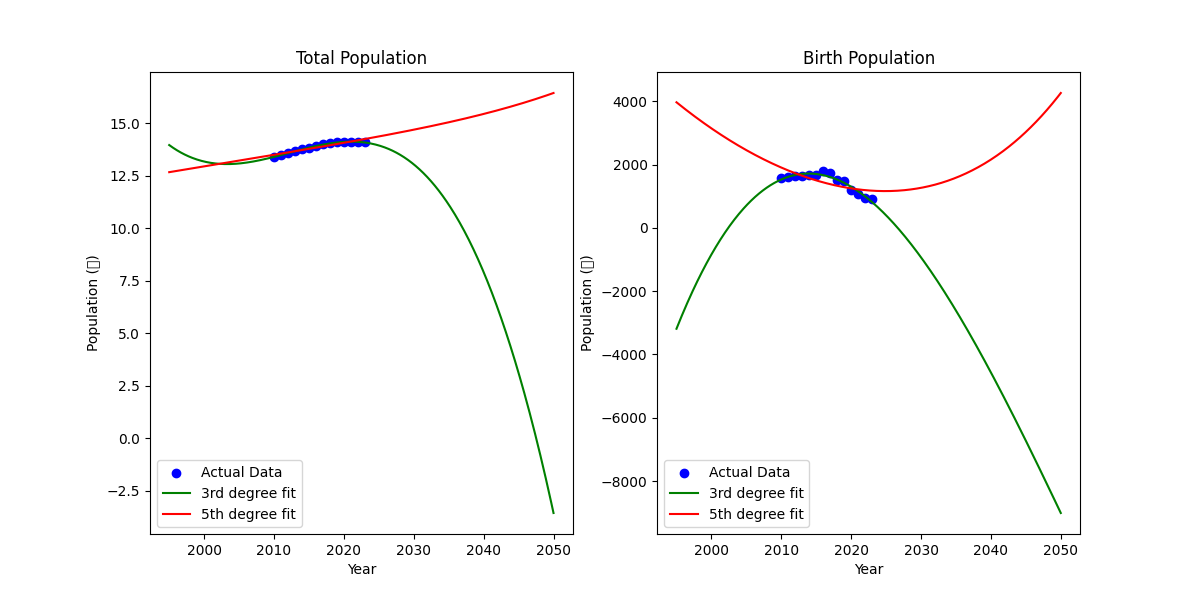
\includegraphics[width=0.8\textwidth]{Figure_1.png}
\end{figure}

\begin{table}[H]
  \begin{tabular}{|c|c|c|c|c|}
    \hline
    预测年份&总人口(亿人)3次&出生人口(万人)3次&总人口(亿人)5次&出生人口(万人)5次\\
    \hline
    2024& 14.036&612.7&14.320&1164.2\\
    \hline
    2030& 13.051&-932.8&14.704&1264.5 \\
    \hline
    2040& 7.915&-4567.2&15.455&2156.5 \\
    \hline
  \end{tabular}
\end{table}

\section{算法分析}
\textcolor{blue}{三次拟合多项式:}

优点:
\begin{itemize}
  \item 模型简单:三次多项式模型复杂度较低,可以避免过拟合。
  \item 稳定性高:适合拟合数据量较少且趋势较平稳的情况,能够捕捉总体变化趋势。
  \item 易于解释:三次曲线常用于描述缓慢变化的非线性趋势,符合人口增长的长期特性。
\end{itemize}
缺点:
\begin{itemize}
  \item 局部拟合能力弱:三次多项式可能无法准确刻画数据的短期波动或复杂变化。
  \item 预测精度有限:对于远期预测,三次多项式容易出现偏差。
\end{itemize}

\textcolor{blue}{次拟合多项式:}

优点:
\begin{itemize}
  \item 灵活性强:五次多项式能更好地拟合复杂的非线性变化,特别是数据点多时,可以捕捉细微波动。
  \item 拟合误差低:拟合时残差较小,能够准确描述现有数据。
\end{itemize}
缺点:
\begin{itemize}
  \item 过拟合风险:五次多项式可能过度关注现有数据的局部特征,导致模型在新数据上的泛化能力差。
  \item 模型复杂性高:高次项的引入可能导致远期预测出现不合理的剧烈变化,违背实际增长规律。
  \item 易受边界影响:对边界点的波动较为敏感,可能导致预测结果偏差较大。
\end{itemize}

\section{结合国情实际的分析}

\textcolor{blue}{中国人口增长现状}
\begin{itemize}
  \item 总人口:

  近年来,中国人口增速放缓,受出生率持续下降影响,总人口增速趋于零甚至开始负增长。
  人口增长符合长期的缓慢变化趋势,过于复杂的模型(如五次多项式)可能会导致预测偏离实际。
  \item   出生人口:

  出生率明显下降,尤其在政策调整和社会经济发展的影响下,呈现波动性减少趋势。
  三次多项式可以反映总体下降趋势,而五次多项式可能会过度拟合导致不合理波动。
  \item  哪种方法更靠谱?
  三次多项式更靠谱:
  三次多项式更能反映总人口和出生人口随时间的平稳变化趋势。由于高次模型(如五次多项式)容易因局部波动或边界效应导致预测值偏离实际,而中国的人口变化趋势较为平稳,因此三次多项式更适合作为人口数据的长期预测模型。
  
\end{itemize}

\section{实验小结}
\textcolor{blue}{结果对比}
\begin{itemize}
  \item 
  拟合效果:
  
  三次多项式模型在拟合精度上稍逊于五次多项式,但在总体趋势的捕捉上表现良好。
  五次多项式模型拟合残差更小,但容易受到边界点的影响,远期预测不稳定。
  \item 预测结果合理性:
  
  三次多项式预测结果更符合中国人口增长的现实趋势,尤其在考虑到未来的低出生率和老龄化趋势时,其预测结果更具参考价值。
  五次多项式的远期预测波动较大,可能出现不切实际的结果。
\end{itemize}

\textcolor{blue}{实验结论}
\begin{itemize}
  \item 
  三次多项式更适合实际应用,能够提供稳定且合理的人口趋势预测,尤其适用于长期政策制定和研究分析。
  \item
  五次多项式可作为补充分析工具,在短期预测或研究数据局部变化时具有一定优势,但需注意避免过拟合。
\end{itemize}

\end{document}
